\documentclass[UTF8,12pt,a4paper]{ctexart}

\usepackage{amsmath,amssymb}
\usepackage{graphicx}
\usepackage{geometry}
\usepackage{setspace}
\usepackage{indentfirst}
\usepackage{fancyhdr}
\usepackage{tocloft}
\usepackage{caption}
\usepackage{float}
\usepackage{booktabs}
\usepackage{array}
\usepackage{multirow}
\usepackage{listings}
\usepackage{xcolor}
\usepackage{chngcntr}
\usepackage[hidelinks]{hyperref}

\hypersetup{bookmarksnumbered=true}

\geometry{left=2.5cm,right=2.5cm,top=2.5cm,bottom=2.5cm}
\setlength{\headheight}{14pt}
\graphicspath{{figure/}}
\setlength{\parindent}{2em}
\onehalfspacing

\ctexset{
    section={
        format=\centering\bfseries\zihao{3},
        aftername=\quad,
        beforeskip=1.0ex,
        afterskip=1.0ex
    },
    subsection={
        format=\bfseries\zihao{4},
        beforeskip=0.8ex,
        afterskip=0.8ex
    }
}

\renewcommand{\contentsname}{目录}
\setcounter{tocdepth}{3}
\setcounter{secnumdepth}{3}
\renewcommand{\cftsecfont}{\normalfont\zihao{4}}
\renewcommand{\cftsubsecfont}{\normalfont\zihao{4}}
\renewcommand{\cftsubsubsecfont}{\normalfont\zihao{-4}}
\renewcommand{\cftsecpagefont}{\normalfont\zihao{4}}
\renewcommand{\cftsubsecpagefont}{\normalfont\zihao{4}}
\renewcommand{\cftsubsubsecpagefont}{\normalfont\zihao{-4}}
\setlength{\cftsecindent}{0em}
\setlength{\cftsubsecindent}{2em}
\setlength{\cftsubsubsecindent}{4em}
\setlength{\cftsecnumwidth}{2.2em}
\setlength{\cftsubsecnumwidth}{3.0em}
\setlength{\cftsubsubsecnumwidth}{3.8em}
\renewcommand{\cftsecleader}{\cftdotfill{\cftdotsep}}
\renewcommand{\cftsubsecleader}{\cftdotfill{\cftdotsep}}
\renewcommand{\cftsubsubsecleader}{\cftdotfill{\cftdotsep}}
\setlength{\cftbeforesecskip}{0.1em}
\setlength{\cftbeforesubsecskip}{0.1em}
\setlength{\cftbeforesubsubsecskip}{0.1em}

\counterwithin{figure}{section}
\counterwithin{table}{section}
\renewcommand{\thefigure}{\thesection-\arabic{figure}}
\renewcommand{\thetable}{\thesection-\arabic{table}}

\captionsetup[figure]{labelfont=bf,textfont=normalfont}
\captionsetup[table]{labelfont=bf,textfont=normalfont}
\captionsetup[lstlisting]{labelfont=bf,textfont=normalfont}

\lstset{
    language=Python,
    basicstyle=\ttfamily\small,
    keywordstyle=\color{blue},
    commentstyle=\color{teal!70!black},
    stringstyle=\color{red!70!black},
    numbers=left,
    numberstyle=\tiny\color{gray},
    stepnumber=1,
    numbersep=6pt,
    frame=single,
    breaklines=true,
    showstringspaces=false,
    tabsize=4,
    captionpos=b
}

\pagestyle{fancy}
\fancyhf{}
\fancyhead[C]{\zihao{5}《人工智能》基于 Transformer 的语音情感特征分析报告}
\fancyfoot[C]{\zihao{5}\thepage}
\renewcommand{\headrulewidth}{0.4pt}
\renewcommand{\footrulewidth}{0pt}

\begin{document}

\zihao{4}

% ==================== 封面 ====================
\begin{titlepage}
    \thispagestyle{empty}

    \noindent
    
\includegraphics[width=7.31cm]{school_logo.png}

    \vspace{2.2cm}

    \begin{center}
        {\zihao{-0}\bfseries 《人工智能》\\[0.5em]基于 Transformer 的语音情感特征分析报告}
    \end{center}

    \vspace{3cm}

    \begin{center}
        {\fangsong\zihao{3}
        \begin{tabular}{rl}
            姓\hspace{2em}名: & 余京航 \\[0.5cm]
            班\hspace{2em}级: & 电子2302班 \\[0.5cm]
            学\hspace{2em}号: & 2306020327 \\[0.5cm]
            专\hspace{2em}业: & 电子信息工程 \\[0.5cm]
            学\hspace{2em}院: & 海洋与空间信息学院
        \end{tabular}

        \vspace{3cm}
        2026 年 5 月 2 日
        }
    \end{center}
\end{titlepage}

% ==================== 目录 ====================
\pagenumbering{Roman}
\phantomsection
\noindent\makebox[\textwidth][c]{\bfseries\zihao{3}目录}\par
\vspace{0.3\baselineskip}
\begingroup
\zihao{4}
\makeatletter
\@starttoc{toc}
\makeatother
\endgroup
\newpage

\pagenumbering{arabic}
\setcounter{page}{1}

% ============================================================
\section{实验目的与任务要求}

\subsection{实验背景}
语音情感识别是语音信号处理与人工智能分类模型结合的典型任务。与文本分类不同，原始语音信号是连续的一维波形，直接输入神经网络会带来较大的计算量，也不利于模型捕获频谱结构。因此，本实验先将语音转换为时序频谱特征，再使用 Transformer Encoder 对时间序列进行建模，最终完成 angry、fear、happy、neutral、sad、surprise 六类中文语音情感分类。

\subsection{实验目的}
本实验围绕“基于 Transformer 的语音情感特征分析”展开，主要目标如下：
\begin{enumerate}
    \item 掌握使用 \texttt{librosa} 加载语音并提取 Mel-spectrogram 或 MFCC 特征的方法。
    \item 编写语音情感数据集类，实现音频样本扫描、标签映射、特征归一化、定长填充与截断。
    \item 理解 Transformer Encoder 中位置编码、多头自注意力和前馈网络对时序特征建模的作用。
    \item 设计语音情感分类器，使用全局平均池化和全连接分类头输出六类情感概率。
    \item 通过训练曲线、验证准确率对比和单文件预测结果分析模型性能与不足。
\end{enumerate}

\subsection{实验环境}
本实验使用 Python 与 PyTorch 完成模型训练和推理，主要依赖如表 \ref{tab:env} 所示。

\begin{table}[H]
\centering
\caption{实验环境与主要工具}
\label{tab:env}
\begin{tabular}{>{\centering\arraybackslash}p{3.5cm}>{\centering\arraybackslash}p{8.5cm}}
\toprule
项目 & 内容 \\
\midrule
编程语言 & Python \\
深度学习框架 & PyTorch \\
音频处理库 & librosa \\
可视化工具 & matplotlib、PyQt \\
特征类型 & Mel-spectrogram，兼容 MFCC \\
训练设备 & CUDA GPU 或 CPU \\
\bottomrule
\end{tabular}
\end{table}

% ============================================================
\section{数据集与语音预处理}

\subsection{CASIA 中文语音情感数据集}
实验数据采用 CASIA 中文语音情感数据集，目录组织形式为“说话人/情感类别/音频文件”。数据集中包含 4 个说话人，每个说话人包含 6 类情感，每类 50 条语音，总计 1200 条样本。六类情感标签及其编号如表 \ref{tab:label-map} 所示。

\begin{table}[H]
\centering
\caption{情感类别与标签编号}
\label{tab:label-map}
\begin{tabular}{>{\centering\arraybackslash}p{3cm}>{\centering\arraybackslash}p{3cm}>{\centering\arraybackslash}p{4cm}}
\toprule
英文标签 & 编号 & 中文含义 \\
\midrule
angry & 0 & 生气 \\
fear & 1 & 害怕 \\
happy & 2 & 开心 \\
neutral & 3 & 平静 \\
sad & 4 & 悲伤 \\
surprise & 5 & 惊讶 \\
\bottomrule
\end{tabular}
\end{table}

\subsection{特征提取方法}
原始语音首先被重采样到 16000 Hz，然后通过短时傅里叶变换得到时频表示。默认特征为 Mel-spectrogram，Mel 滤波器个数为 64，帧移为 160，窗长为 400，FFT 点数为 1024。Mel 频谱计算后进一步转换为对数能量形式：
\begin{equation}
S_{db}=10\log_{10}(S+\epsilon)
\end{equation}
其中 $S$ 表示 Mel 能量谱，$\epsilon$ 用于避免对零取对数。对数 Mel 特征更接近人耳对响度的感知方式，也能压缩动态范围，使网络训练更加稳定。

\subsection{定长序列处理}
Transformer 需要批量处理形状一致的输入序列。本实验将每条语音的特征统一为 $L=300$ 帧。当语音帧数不足 300 时，在末尾补零并生成有效帧掩码；当语音帧数超过 300 时，在训练阶段使用随机裁剪，在验证阶段使用居中裁剪。处理后单条样本形状为：
\begin{equation}
X\in \mathbb{R}^{300\times 64}
\end{equation}
其中 300 表示时间帧数，64 表示每帧 Mel 特征维度。

\subsection{数据增强策略}
为了提升训练阶段的鲁棒性，数据集类在训练模式下加入了 SpecAugment 思想，对频率维度和时间维度进行随机遮挡。此外，代码中还实现了加性高斯噪声和音量扰动方法，可用于模拟真实语音环境中的噪声和录音强度变化。数据增强只作用于训练集，验证集保持原始特征，以保证评估结果可比。

% ============================================================
\section{Transformer 情感分类模型设计}

\subsection{整体模型结构}
本实验构建的 \texttt{TransformerEmotionClassifier} 由输入投影层、位置编码、Transformer Encoder、LayerNorm、全局平均池化和线性分类头组成。模型整体流程如下：
\begin{equation}
\text{Logits}=\text{Linear}\left(\text{Pool}\left(\text{TransformerEncoder}\left(\text{PE}\left(\text{Linear}(X)\right)\right)\right)\right)
\end{equation}

\begin{table}[H]
\centering
\caption{模型主要超参数}
\label{tab:model-params}
\begin{tabular}{>{\centering\arraybackslash}p{4cm}>{\centering\arraybackslash}p{4cm}>{\centering\arraybackslash}p{4cm}}
\toprule
参数 & 取值 & 说明 \\
\midrule
输入维度 & 64 & Mel 特征维度 \\
\texttt{d\_model} & 128 & Transformer 隐藏维度 \\
\texttt{nhead} & 4 & 多头注意力头数 \\
\texttt{num\_layers} & 3 & Encoder 层数 \\
\texttt{ffn\_dim} & 256 & 前馈网络隐藏维度 \\
\texttt{dropout} & 0.15 & 随机失活比例 \\
输出类别数 & 6 & 六类情感 \\
\bottomrule
\end{tabular}
\end{table}

\subsection{位置编码}
由于 Transformer 的自注意力机制本身不包含序列顺序信息，因此需要为每个时间帧加入位置编码。本实验使用标准正弦位置编码：
\begin{equation}
PE_{(pos,2i)}=\sin\left(\frac{pos}{10000^{2i/d_{model}}}\right)
\end{equation}
\begin{equation}
PE_{(pos,2i+1)}=\cos\left(\frac{pos}{10000^{2i/d_{model}}}\right)
\end{equation}
其中 $pos$ 表示时间位置，$i$ 表示特征维度索引。该编码能为模型提供相对和绝对时序位置信息，使模型能够区分语音中不同时间片段的先后关系。

\subsection{多头自注意力机制}
Transformer Encoder 的核心是多头自注意力。对于输入序列 $X$，模型分别计算查询矩阵 $Q$、键矩阵 $K$ 与值矩阵 $V$，注意力输出为：
\begin{equation}
\text{Attention}(Q,K,V)=\text{softmax}\left(\frac{QK^T}{\sqrt{d_k}}\right)V
\end{equation}
多头机制将特征空间划分为多个子空间并行建模，使模型能够同时关注语音中的不同情感线索，例如能量变化、局部频谱结构和长时依赖关系。

\subsection{分类头设计}
Transformer Encoder 输出的每一帧仍然是时序表示。为了得到整条语音的情感类别，本实验对有效帧进行掩码平均池化：
\begin{equation}
h=\frac{\sum_{t=1}^{L}m_t h_t}{\sum_{t=1}^{L}m_t}
\end{equation}
其中 $m_t$ 为有效帧掩码，补零帧不参与平均。最后通过线性层将全局语音表示映射到六类情感 logits，再使用交叉熵损失训练。

\newpage
% ============================================================
\section{训练方法与评估设置}

\subsection{训练流程}
训练过程包括数据扫描、标签映射、训练/验证划分、特征提取、模型前向传播、损失计算、反向传播和模型保存。核心训练参数如表 \ref{tab:train-params} 所示。

\begin{table}[H]
\centering
\caption{训练参数设置}
\label{tab:train-params}
\begin{tabular}{>{\centering\arraybackslash}p{4cm}>{\centering\arraybackslash}p{4cm}>{\centering\arraybackslash}p{4cm}}
\toprule
参数 & 取值 & 说明 \\
\midrule
优化器 & AdamW & 带权重衰减的自适应优化 \\
学习率 & $3\times10^{-4}$ & 初始学习率 \\
batch size & 16 & 单批样本数 \\
最大 epoch & 100 & 最大训练轮数 \\
weight decay & $5\times10^{-4}$ & 权重衰减 \\
label smoothing & 0.1 & 缓解过拟合和过度自信 \\
梯度裁剪 & 1.0 & 限制梯度范数 \\
早停耐心轮数 & 12 & 验证准确率长期不提升则停止 \\
\bottomrule
\end{tabular}
\end{table}

\subsection{两种验证划分方式}
为了更全面地分析模型性能，本实验采用两种划分方式：按情感类别分层随机划分和按说话人留出划分。二者的区别如表 \ref{tab:split} 所示。

\begin{table}[H]
\centering
\caption{两种验证划分方式对比}
\label{tab:split}
\begin{tabular}{>{\centering\arraybackslash}p{3cm}>{\centering\arraybackslash}p{4cm}>{\centering\arraybackslash}p{3cm}>{\centering\arraybackslash}p{3cm}}
\toprule
模式 & 划分方式 & 验证集规模 & 难度 \\
\midrule
按情感划分 & 每类随机 8:2 分层 & 240 条 & 较低 \\
按说话人划分 & 留出 1 个完整说话人 & 300 条 & 较高 \\
\bottomrule
\end{tabular}
\end{table}

按情感划分时，同一说话人的语音可能同时出现在训练集和验证集中，因此模型更容易学习到说话人相关的音色特征。按说话人划分时，验证集来自训练阶段未见过的说话人，更能检验模型跨说话人的泛化能力，因此难度明显更高。

\newpage
% ============================================================
\section{实验结果与分析}

\subsection{训练曲线分析}
图 \ref{fig:training-curves} 展示了模型训练过程中的损失和准确率变化。按情感划分模式下，训练准确率从 0.3417 提升到 0.8781 左右，验证准确率最高达到 1.050，最佳轮次为第 19 轮。之后训练准确率继续保持较高水平，但验证准确率出现波动，说明模型已经学习到主要情感区分特征，同时也开始受到数据规模和说话人差异的影响。

\begin{figure}[H]
    \centering
    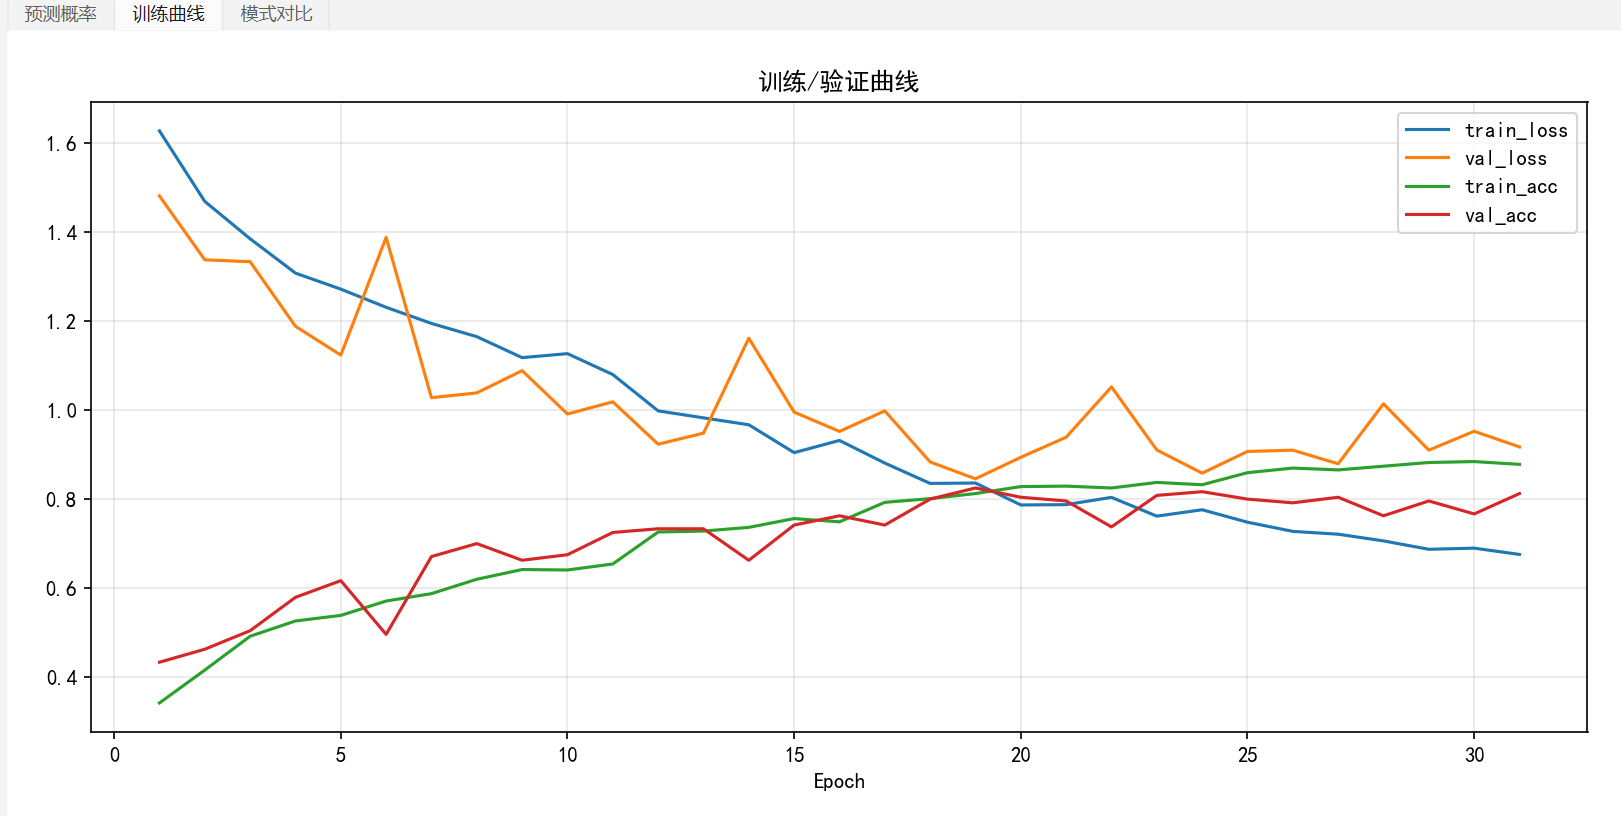
\includegraphics[width=1.0\textwidth]{训练验证曲线.png}
    \caption{训练与验证曲线}
    \label{fig:training-curves}
\end{figure}

从曲线变化可以看出，训练损失整体下降，训练准确率稳定上升，说明模型具备有效拟合训练集的能力。验证曲线在中后期存在一定震荡，主要原因包括：CASIA 数据集规模较小、每类样本数量有限、不同情感之间存在语音表达相似性，以及随机裁剪和 SpecAugment 带来的训练扰动。总体上，按情感划分下的验证准确率已经显著高于六分类随机猜测水平 $1/6\approx16.67\%$。

\subsection{两种划分模式对比}
图 \ref{fig:split-compare} 对比了按情感划分和按说话人划分两种模式的验证准确率。按情感划分的最佳验证准确率为 82.50\%，而按说话人划分的最佳验证准确率约为 41.33\%。

\begin{figure}[H]
    \centering
    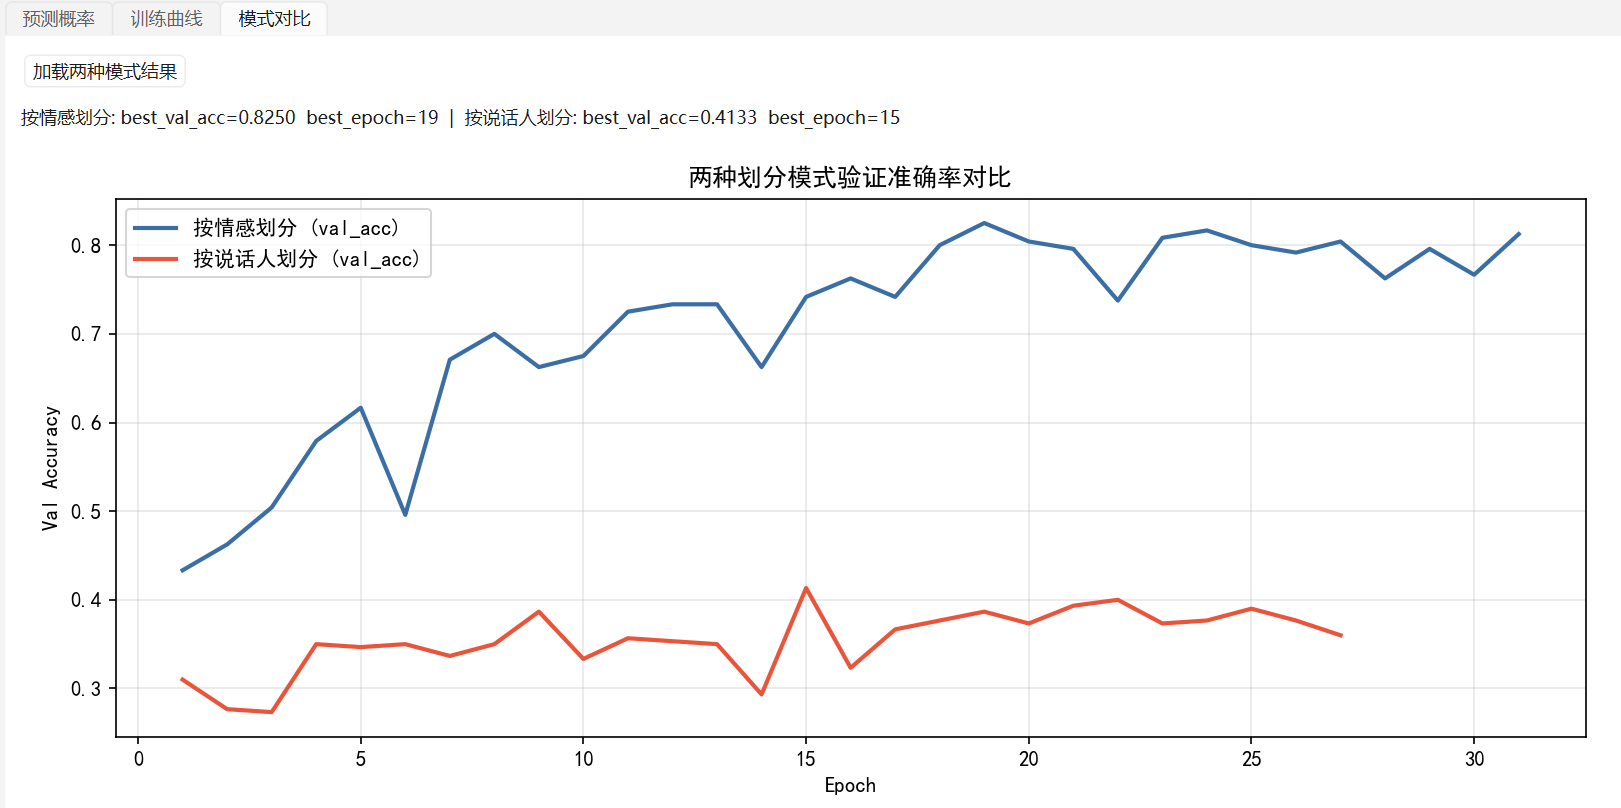
\includegraphics[width=1.0\textwidth]{两种划分模式验证准确率对比.png}
    \caption{两种划分模式验证准确率对比}
    \label{fig:split-compare}
\end{figure}

该结果说明，模型在“同分布、说话人部分重合”的验证场景下能够取得较高准确率，但在面对完全未见过的说话人时性能明显下降。造成该现象的主要原因有三点：
\begin{enumerate}
    \item \textbf{说话人音色差异明显}：不同说话人的音高、语速、发音习惯和能量分布不同，模型容易把部分说话人特征误当作情感特征。
    \item \textbf{数据规模较小}：每类每个说话人只有 50 条样本，模型难以充分学习跨说话人的稳定情感表达模式。
    \item \textbf{外部泛化更困难}：按说话人划分更接近真实应用场景，要求模型忽略身份差异并捕获情感共性，因此验证准确率更低是合理现象。
\end{enumerate}

因此，两种划分模式的准确率不能直接作为同一难度下的性能对比。按情感划分主要反映模型对当前数据集内部样本的拟合能力，按说话人划分则更能反映泛化能力。

\subsection{训练集样例预测结果}
为验证模型对已学习分布内样本的识别效果，选取训练数据集中 angry 与 fear 类别语音进行单文件预测。预测结果如图 \ref{fig:angry-predict} 和图 \ref{fig:fear-predict} 所示。

\begin{figure}[H]
    \centering
    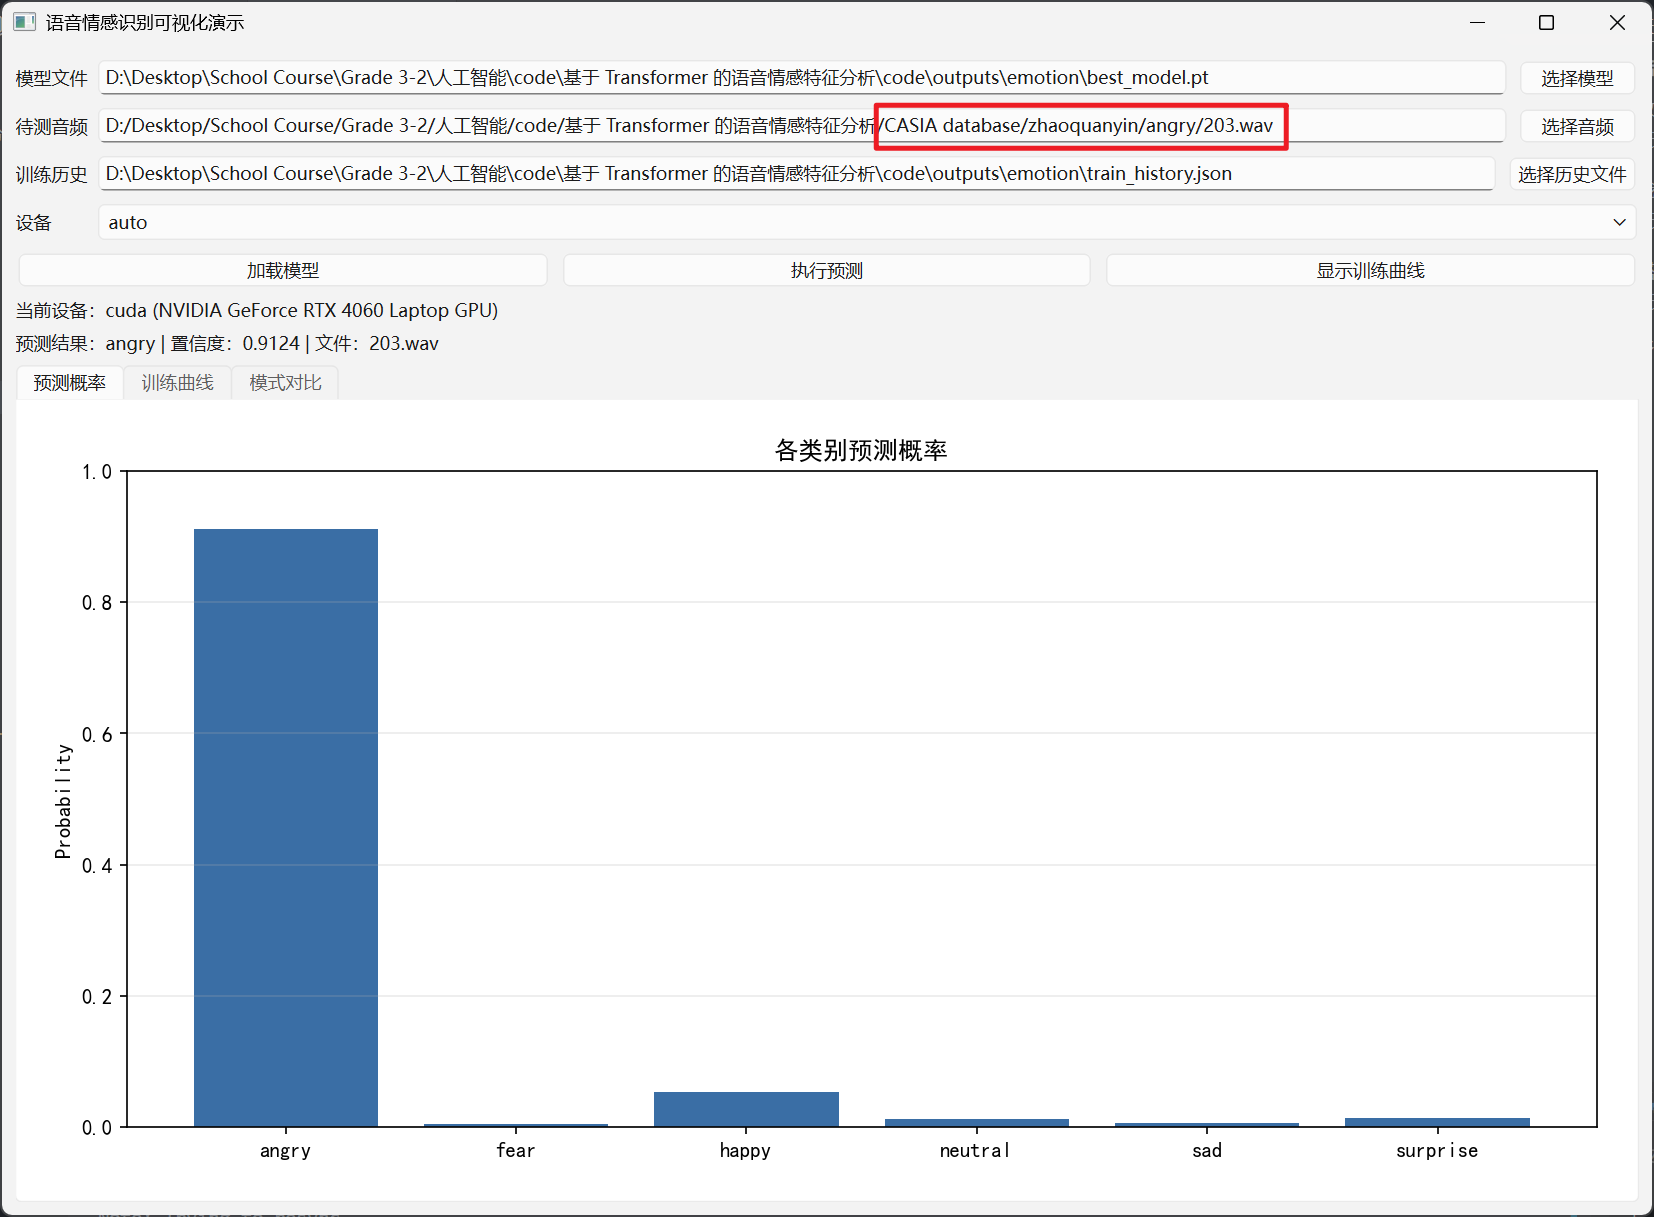
\includegraphics[width=0.9\textwidth]{用训练的数据集测试angry.png}
    \caption{训练数据集中 angry 样本预测结果}
    \label{fig:angry-predict}
\end{figure}

\begin{figure}[H]
    \centering
    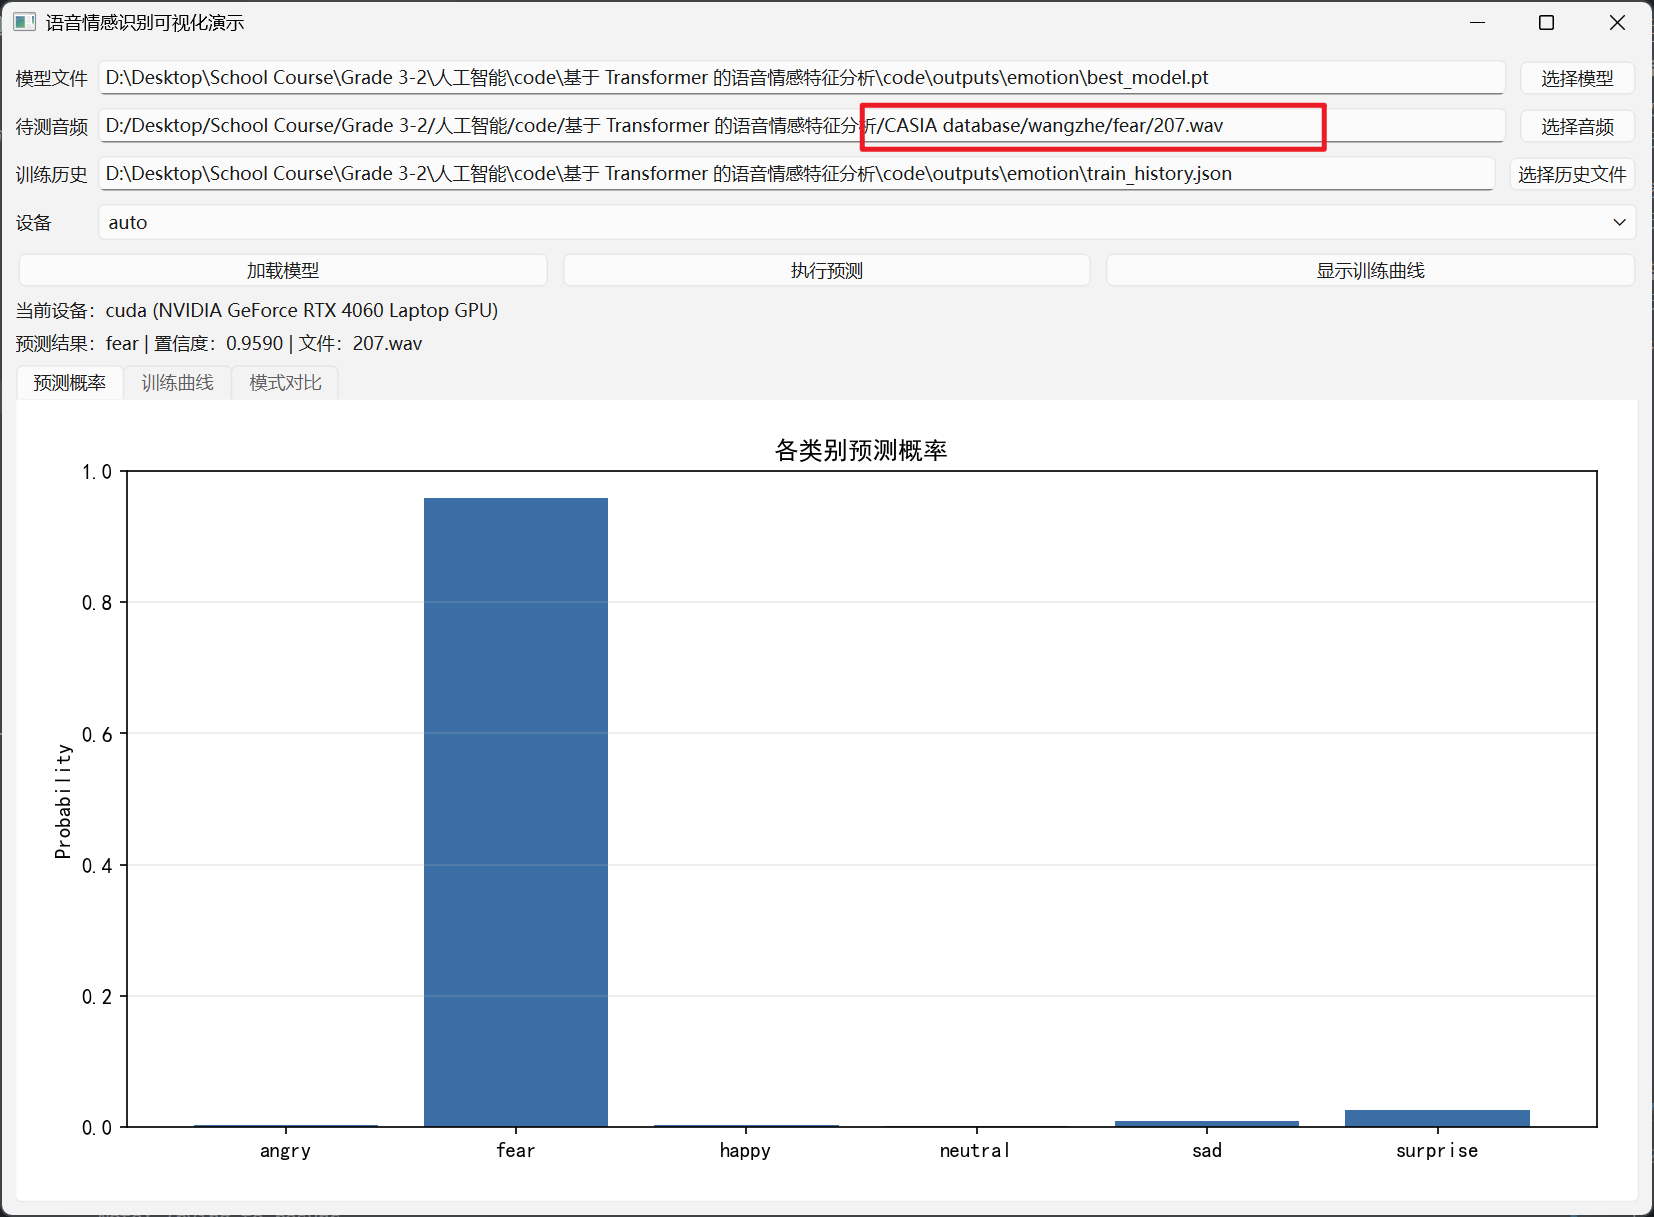
\includegraphics[width=0.9\textwidth]{用训练的数据集测试fear.png}
    \caption{训练数据集中 fear 样本预测结果}
    \label{fig:fear-predict}
\end{figure}

从训练集样例结果可以看出，模型对数据集内部语音具有较明确的类别判断，目标类别概率通常明显高于其他类别。这表明模型能够从 Mel-spectrogram 中学习到与情感相关的时序频谱模式。例如 angry 语音往往具有更强的能量和更明显的频谱变化，fear 语音在声调和能量波动上也具有一定差异。由于这些样本与训练集同源，录音环境、说话方式和文本内容较一致，因此识别效果相对稳定。

\subsection{外部素材预测结果}
为了进一步观察模型在非标准数据上的表现，实验还选取了“鸡汤来了”和“臣妾做不到”等外部语音素材进行预测，结果如图 \ref{fig:happy-material} 和图 \ref{fig:sad-material} 所示。

\begin{figure}[H]
    \centering
    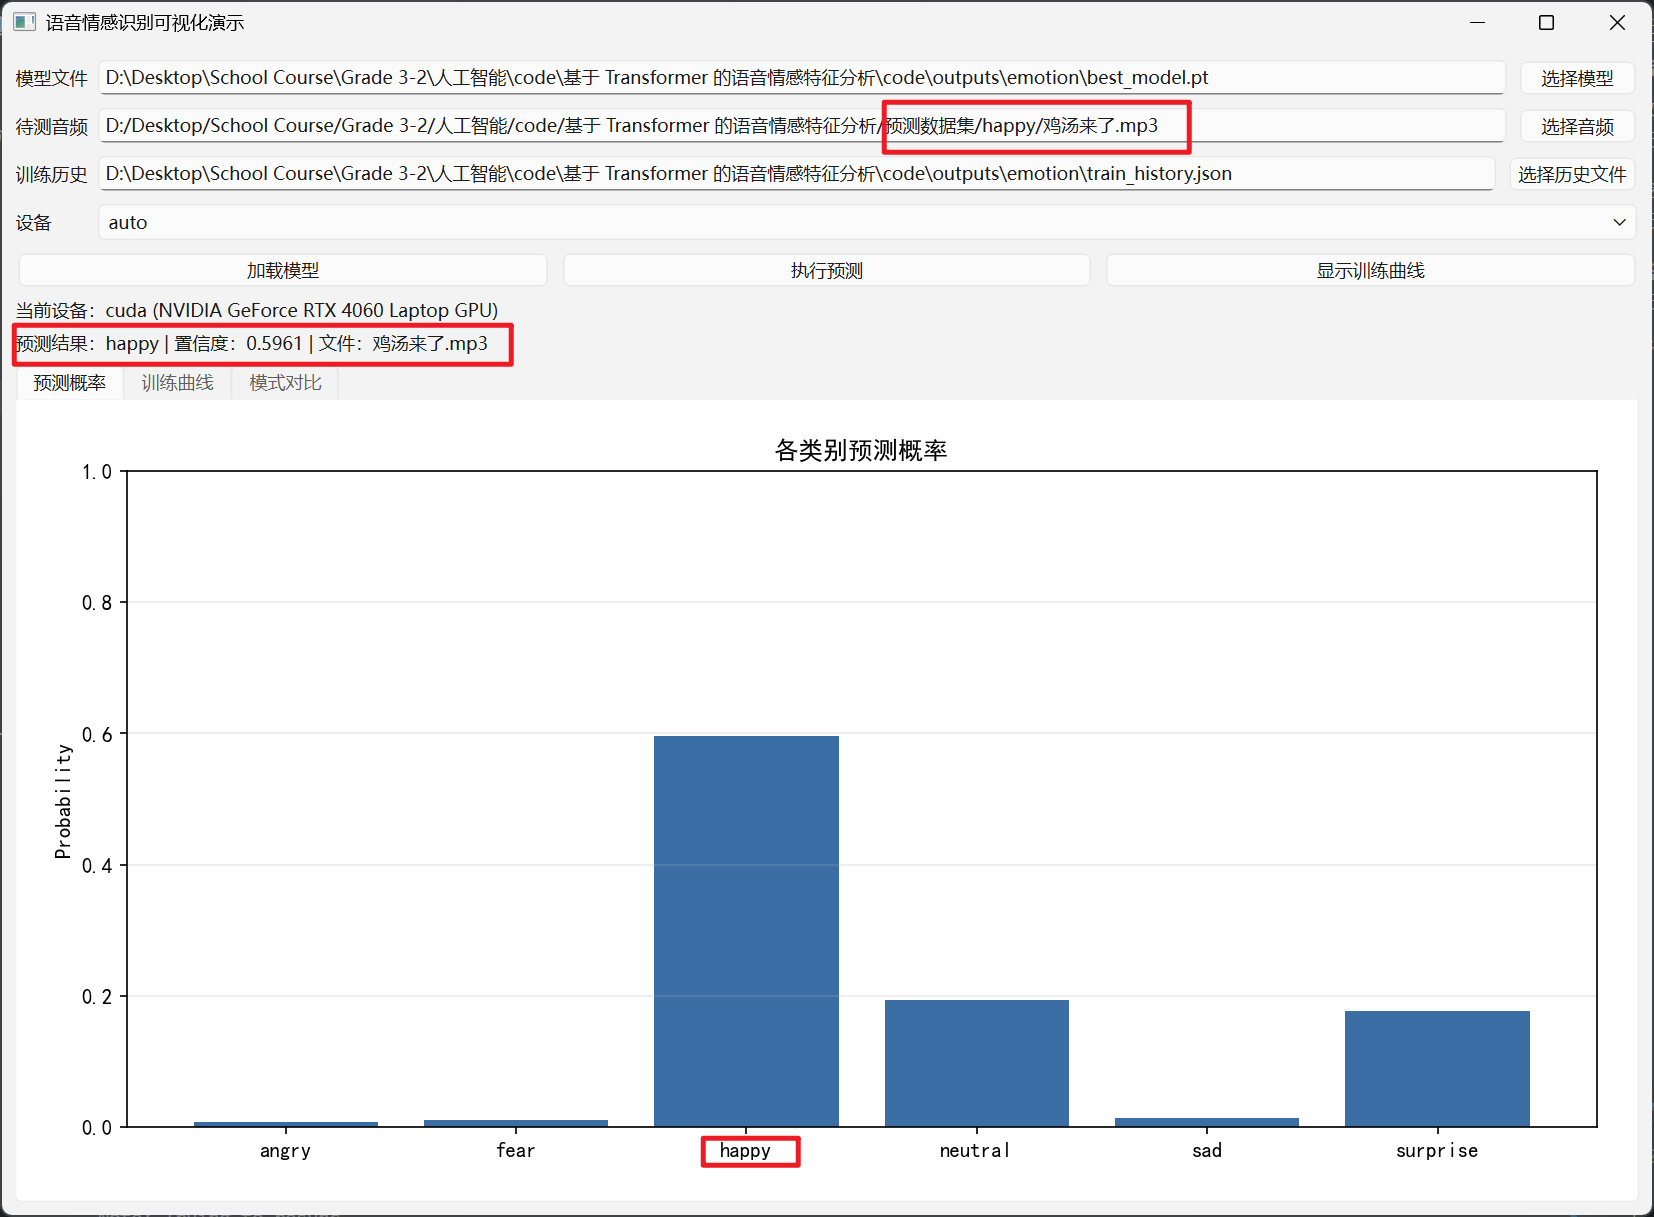
\includegraphics[width=0.9\textwidth]{鸡汤来了素材happy.png}
    \caption{外部素材 happy 倾向预测结果}
    \label{fig:happy-material}
\end{figure}

\begin{figure}[H]
    \centering
    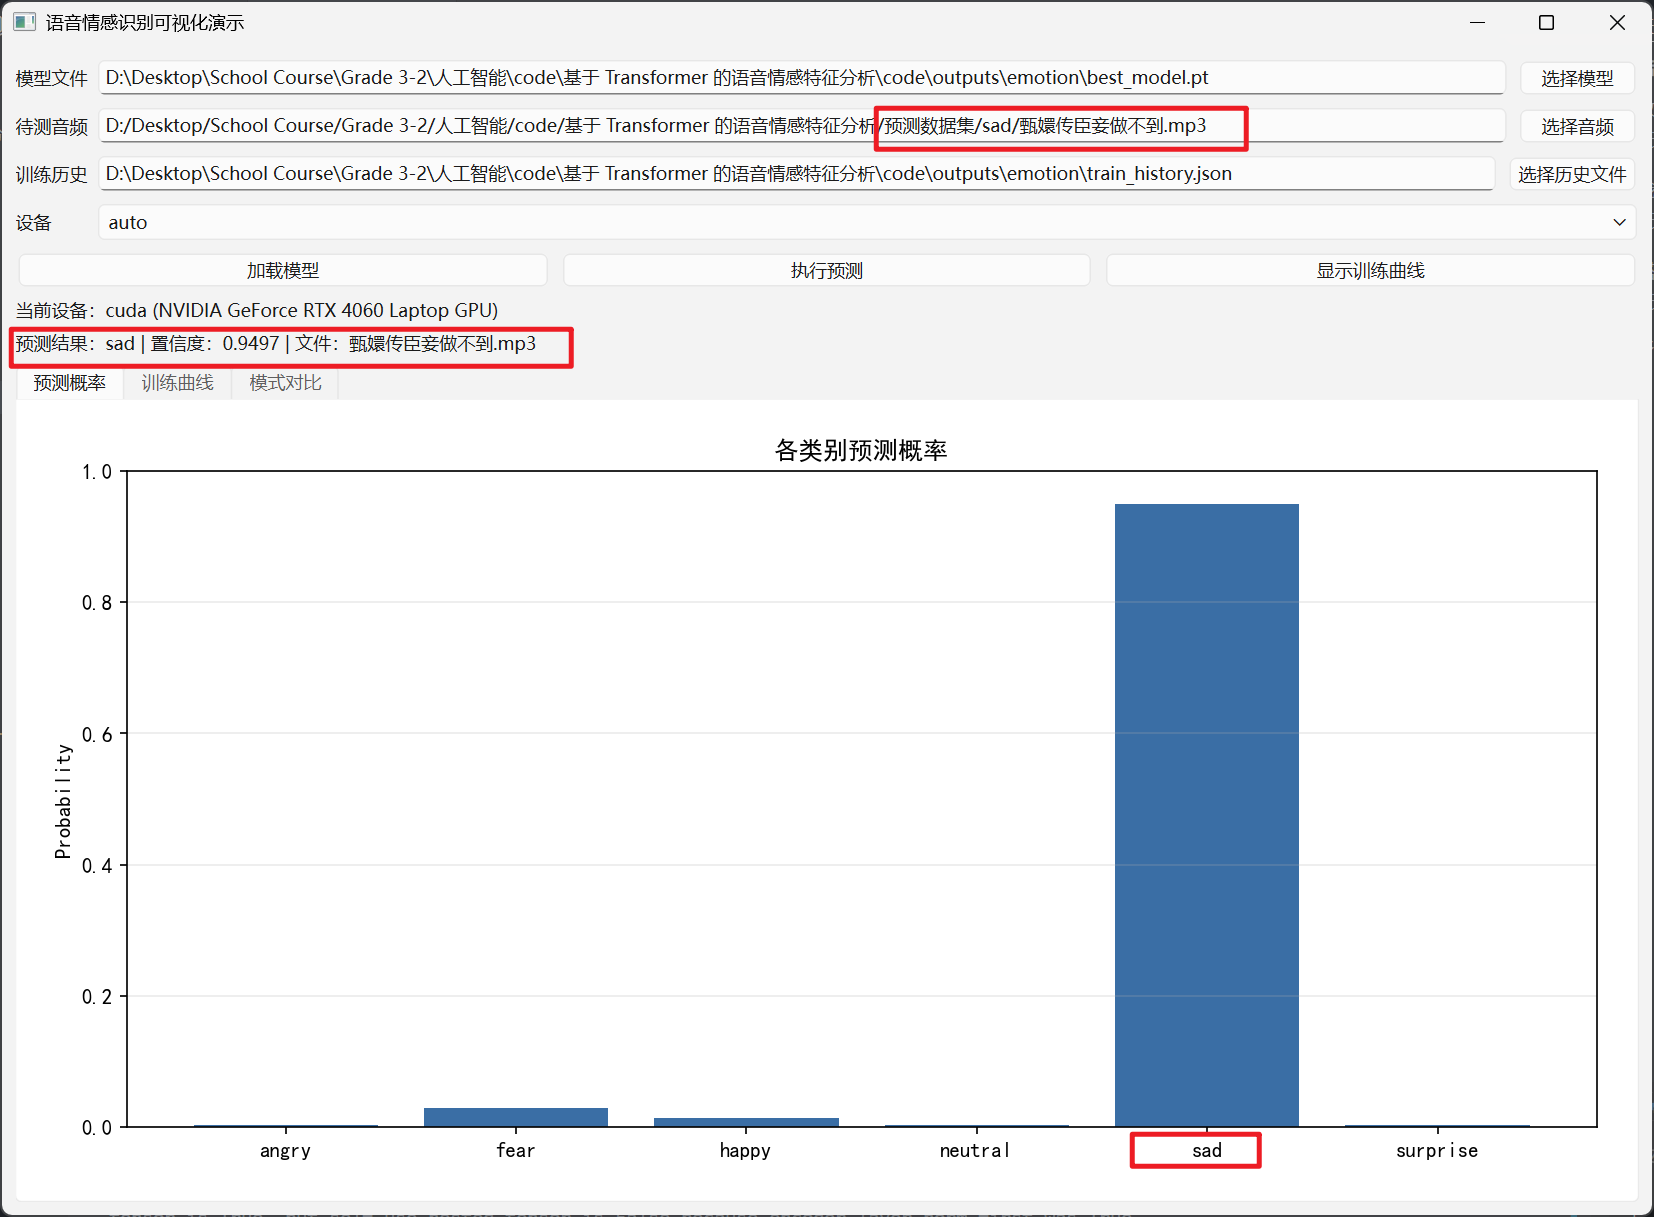
\includegraphics[width=0.9\textwidth]{臣妾做不到素材sad.png}
    \caption{外部素材 sad 倾向预测结果}
    \label{fig:sad-material}
\end{figure}

外部素材与 CASIA 数据集存在明显域差异，包括录音设备、背景噪声、语速、语调夸张程度、文本内容和说话人身份等。因此，外部预测结果更适合作为定性演示，而不应与验证集准确率直接等同。若模型在外部素材上仍能给出符合直觉的情感倾向，说明其学习到了一部分可迁移的声学情感线索；若预测概率分布较分散或出现误判，也反映出模型对真实复杂语音的泛化能力仍有限。

\subsection{结果总结}
综合训练曲线、验证准确率和预测样例，可以得到以下结论：
\begin{enumerate}
    \item Transformer Encoder 能够有效处理 Mel-spectrogram 时序特征，并完成六类语音情感分类。
    \item 按情感划分时，模型最高验证准确率达到 82.50\%，说明在数据集内部划分下分类效果较好。
    \item 按说话人划分时，最高验证准确率约为 41.33\%，说明跨说话人泛化是本任务的主要难点。
    \item 训练集样例预测较稳定，外部素材预测受域差异影响更大，体现出实际应用中需要更多数据增强和跨域训练。
\end{enumerate}

% ============================================================
\section{关键代码说明}

\subsection{特征提取与定长处理}
数据集部分的核心逻辑是先提取音频特征，再统一时间长度。其简化流程如下：

\begin{lstlisting}[caption={语音特征提取与定长处理流程}]
waveform, _ = librosa.load(str(wav_path), sr=16000)
feature = librosa.feature.melspectrogram(
    y=waveform,
    sr=16000,
    n_mels=64,
    n_fft=1024,
    hop_length=160,
    win_length=400,
)
feature = librosa.power_to_db(feature, ref=1.0)
feature = feature.T.astype(np.float32)
feature = (feature - feature.mean()) / (feature.std() + 1e-6)
feature, valid_mask = pad_or_truncate(feature, target_len=300)
\end{lstlisting}

该流程将不同长度的原始语音转换为统一形状的二维特征矩阵，并通过 \texttt{valid\_mask} 标记真实帧位置，使后续池化时不会把补零帧计入平均。

\subsection{模型前向传播}
模型前向传播的关键在于输入投影、位置编码、掩码注意力和有效帧池化。简化代码如下：

\begin{lstlisting}[caption={Transformer 情感分类器前向传播}]
x = self.input_projection(x)
x = self.position_encoder(x)

src_key_padding_mask = None
if valid_mask is not None:
    src_key_padding_mask = ~valid_mask.bool()

encoded = self.transformer_encoder(
    x,
    src_key_padding_mask=src_key_padding_mask,
)
encoded = self.final_norm(encoded)

mask = valid_mask.unsqueeze(-1).to(dtype=encoded.dtype)
pooled = (encoded * mask).sum(dim=1) / mask.sum(dim=1).clamp_min(1.0)
logits = self.classifier(pooled)
\end{lstlisting}

其中 \texttt{src\_key\_padding\_mask} 用于避免 Transformer 关注补零帧，掩码平均池化则保证分类向量只来自真实语音片段。

% ============================================================
\section{问题分析与改进方向}

\subsection{存在问题}
实验结果表明，当前模型已经能够完成基本的语音情感分类，但仍存在以下不足：
\begin{enumerate}
    \item \textbf{跨说话人泛化不足}：按说话人划分准确率明显低于按情感划分，说明模型对说话人特征仍较敏感。
    \item \textbf{数据规模有限}：CASIA 数据集中说话人数量和样本数量较少，难以覆盖真实场景中的语音变化。
    \item \textbf{外部音频域偏移明显}：网络素材的录音环境、音质和表达方式与训练集差异较大，预测结果稳定性下降。
    \item \textbf{情感边界模糊}：部分情感在声学特征上相似，例如 fear 与 surprise、sad 与 neutral，容易产生混淆。
\end{enumerate}

\subsection{改进方向}
后续可从以下方面继续优化：
\begin{enumerate}
    \item 增加更多说话人和真实场景语音数据，提升模型对说话人差异和录音环境变化的鲁棒性。
    \item 引入更强的数据增强策略，如混响模拟、背景噪声叠加、速度扰动和音高扰动。
    \item 尝试预训练语音模型，如 wav2vec 2.0、HuBERT 等，以利用大规模无标注语音中的通用表征。
    \item 在损失函数或采样策略中加入类别混淆约束，提高相近情感之间的区分能力。
    \item 结合文本内容、语音能量统计和韵律特征，构建多特征融合的情感识别系统。
\end{enumerate}

% ============================================================
\section{实验总结}

本实验完成了一个基于 Transformer 的中文语音情感分类系统。实验首先使用 \texttt{librosa} 将原始语音转换为 Mel-spectrogram，并通过填充、截断和掩码机制构造固定长度输入；随后使用正弦位置编码和 Transformer Encoder 对时序频谱特征进行建模；最后通过全局平均池化和线性分类头实现六类情感识别。

从实验结果看，模型在按情感随机划分场景下取得了较好的验证准确率，说明 Transformer 能够从频谱序列中学习有效的情感特征；但在按说话人划分时准确率下降明显，说明跨说话人泛化仍是语音情感识别任务中的关键挑战。外部素材预测进一步说明，真实应用场景中还需要考虑数据域偏移、噪声、录音设备和表达方式差异等问题。

总体而言，本实验完整覆盖了语音预处理、Transformer 建模、训练评估和预测演示流程，加深了对语音情感特征分析和深度学习时序分类方法的理解。

\end{document}
